\documentclass[a4paper]{article}

\usepackage{listings}
\usepackage{graphicx}
\usepackage{fancyhdr}
\usepackage{color}
\usepackage{xcolor}
\pagestyle{fancy}

\lhead{Tube Tracker}
\rhead{CSN08113}
\lfoot{Final Report}
\cfoot{\thepage}
\rfoot{Gareth Pulham, 40099603}

\lstdefinestyle{customc}{
    belowcaptionskip=1\baselineskip,
    frame=single,
    xleftmargin=\parindent,
    language=C,
    showstringspaces=false,
    basicstyle=\footnotesize\ttfamily,
    keywordstyle=\bfseries\color{green!40!black},
    commentstyle=\itshape\color{purple!40!black},
    identifierstyle=\color{blue},
    stringstyle=\color{orange},
}


\begin{document}
    \begin{titlepage}
        \title{Physical Computing CSN08113\\
            Tube Tracker
        }
        \author{Gareth Pulham, 40099603}
        \date{\today}
        \maketitle
        \thispagestyle{empty}

        \begin{abstract}
            This project aims to produce a ``Tube Tracker'', a device which can be used to identify the location of a catheter inside the body by detecting the metal guide wire when placing it.
            To do so, the device interprets signals produced by a COTS metal detector commonly used for security purposes.

            By examining and measuring the metal detectors internal construction, it was possible to identify and interpret the strength of metal detection, which can then be displayed to the user to deduce the location of the guide wire.

            As a result of this work, a working prototype was developed and demonstrated.

            This project was undertaken in partnership with Megan Currie, a product design student at Edinburgh Napier University, who developed the concept and packaging for this project.
        \end{abstract}
    \end{titlepage}

    \tableofcontents

    \section{Introduction}
    Surgery and other clinical procedures are under ever increasing pressure to be able to up their effectiveness, complete more radical and effective procedures, and treat previously unreachable parts of the body, while at the same time continuously decrease their invasiveness and other adverse impacts on the patient. These pressures have led to continous innovation in medical technology, with one of the most significant jumps being the introduction of laparoscopy, also known as keyhole surgery, where only a tiny incision is made, and all tools are operated on flexible stalks passed through this small hole, with navigation being done by camera.

    There are other instances in the clinical setting where we want to execute minimally invasive procedures, and have to accept that this means a more challenging working environment, such as not being able to see the tools in use, and a subfield of computer-assisted surgery, `surgical navigation', has sprung up around this, providing better insight into the position and manoeuvring of tools.

    This project aims to be the first part of a wider ``Swiss Army Nurse'' project, a collection of many useful nursing tools in a handheld package. This component is a simple navigation tool to help nurses identify the location of a catheter as it's being inserted, a simple procedure but which requires some practice in inexperienced nurses to ensure that the tube follows the correct path as it's being inserted.

    \section{Deliverables}
    \begin{itemize}
        \item Prototype Tube Tracker
        \item Final Report (this document)
    \end{itemize}

    \section{Design}
        \subsection{Sensor Types}
        The mode of operation of medical navigation falls into five broad categories:
        \begin{itemize}
            \item Optical
            \item Electromechanical
            \item Electromagnetic
            \item Ultrasonic
            \item and Radiological
        \end{itemize}
        For the purposes of this project, radiological sensing is not considered a viable option due to it's highly controlled distribution and the impact it has on patients and operators, amongst other reasons.

        An optically guided solution would also not be suitable for this project, as it depends on a number of preparatory steps, such as registering a 3D model of the operating area. Additionally, they are most effective with rigid tools, unlike the catheter that this project aims to use.

        This leaves three remaining options: ultrasonic, electromagnetic, and electromechanical.

            \subsubsection{Ultrasonic}
            Ultrasonic sensing relies on sending high frequency sound ``chirps'' into the body, and then analysing the echos reflected by tissue structures or other objects that the chirps strike. It has a proven track record, and is used daily in a range of settings, from routine obstretic imaging to emergency medical teams providing trauma care.

            Ultrasound also has a relatively low training cost compared to other sensing methods such as radiological and optical, but it does have overhead in preparing a patient for imaging - the area where the image is to be taken must be cleared of obstructions (dirt, hair, etc) and the application of gel to improve conductivity.

            The real challenge to implement ultrasonic in this project is however is that ultrasound requires sophisiticated signal processing capabilities to turn the returned echoes into an understandable image. Additionally, it will be difficult to differentiate the catheter from other body tissues (searching for a metal wire behind the sternum\slash in front of the spine, inside of an airspace).

            \subsubsection{Electromagnetic}
            Electromagnetic sensing in this instance would be possible as we are essentially operating as a metal detector to find the guidewire inserted into the catheter.

            \subsubsection{Electromechanical}
            Electromechanical navigation is where the catheter tip can be instrumented with accelerometers/gyros, and we can measure the motion recorded on these the same way as used in INS. By continually integrating these accelerations over time we can get speed, and integrating again gives us a displacement from where the measurements were started.

            Again there are downsides to this method, in particular, single-use elements have to be instrumented with expensive parts which then cannot be reused. Additionally, like optical systems, for the best results, the area where the device will be used should be pre-registered.

    \section{Schematic}
    \begin{figure}[h]
        \centering
        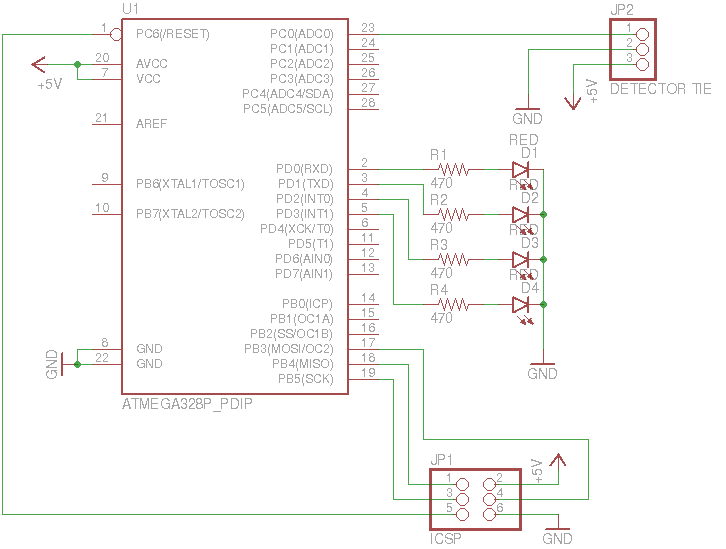
\includegraphics[width=0.75\textwidth]{images/schematic}
        \caption{It's the schematics}
    \end{figure}

    \section{Source}
    \lstinputlisting[style=customc]{../src/tracker.c}

\end{document}
